\section{Introduction}
The world wide web is by far the largest source of information today.
Much of that information contains structured data such as tables and lists
which are very valuable for knowledge discoverage and data mining. 
This structured data is valuable not only because of the relational
values it contains, but also because it is relatively easier to unlock
information from data with some regular patterns than free text which
makes up most of the web content. However, when encoded in HTML, 
structured data becomes {\em semi-structured}. 
And because HTML is designed for rendering in a browser, different
HTML code segments can give the same visual effect at least to
the human eye. As a result, 
HTML coding is much less stringent than XML, and
inconsistencies and errors are abundant in HTML documents. 
All these pose significant challenges in the extraction of structured 
data from the web \cite{Weninger10:UnexpectedList}.

In this demo, we focus on list data in web pages. In particular, we are 
interested in extracting from a kind of web pages which present
a list of $k$ instances of a topic or a concept. Examples of such topic include 
``20 Most Influential Scientists Alive Today'', 
``Ten Hollywood Classics You Shouldn't Miss'', 
``50 Tallest Persons in the World''. Figure \ref{fig:topscientists}.(a)
shows a snapshot of one such web page \cite{InfluentialScientists}.

\begin{figure*}[th]
        \centering
        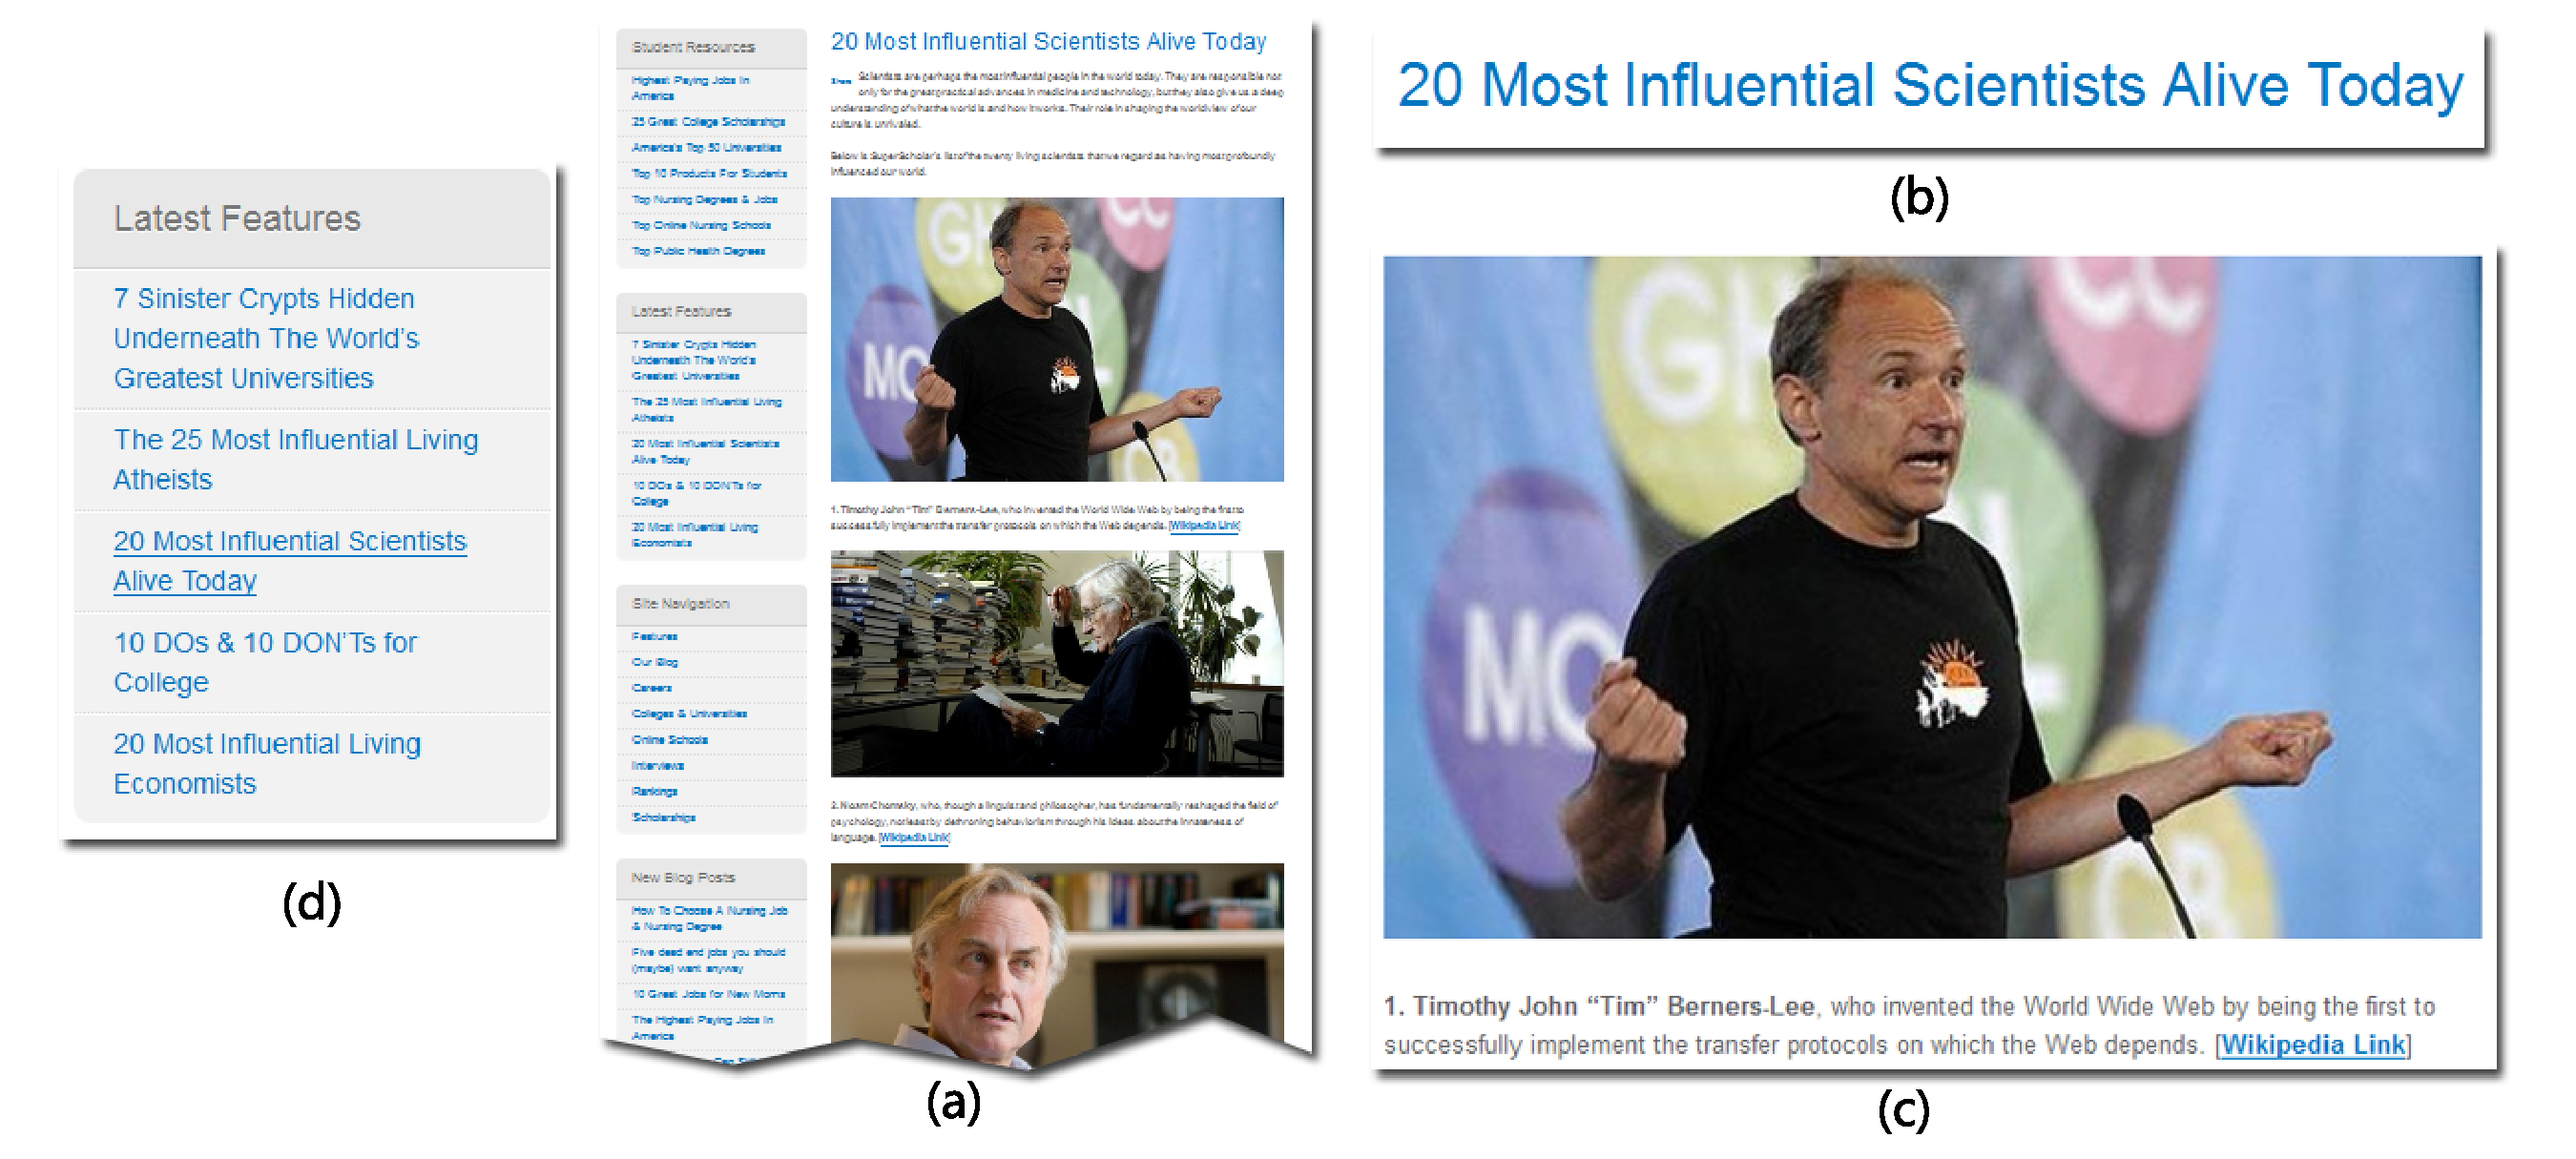
\epsfig{file=./pic/page5_detail.eps,width=1.8\columnwidth}
        \caption{Snapshot of a typical {\em top-k page} and its page segments}
        \label{fig:topscientists}
\end{figure*}

%\begin{figure}[th]
%	\centering
%	\epsfig{file=./pic/page5.eps, width=0.75\columnwidth}
%	\caption{Snapshot of a typical {\em top-k page}}
%	\label{fig:topscientists}
%\end{figure}

Informally, our problem is: given a web page with a title that contains
a integer number $k$ (Figure \ref{fig:topscientists}.(b)), 
check whether the page contains a list of $k$ items
as its {\em main content}, and if it does, extract these $k$ items. 
We call such lists {\em top-k lists} and pages that contain the 
entirety of a top-k list {\em top-k pages}. 
There are also lists that span multiple pages but are connected by 
hyperlinked ``Next'' button,
%such as the page \cite{TopFootball} shown in Figure \ref{fig:multipagelist},
but these are not considered in this work. 
A typical scenario we consider, 
like the one in Figure \ref{fig:topscientists}, is that
each list item is more than an instance of the topic in the title, 
but instead contain additional information such as 
a textual description and images, like in Figure \ref{fig:topscientists}.(c). 
Our objective is to extract the actual instance whenever possible, 
but in the worst case, produce list items that at least {\em contain} 
the wanted instances.

%\begin{figure}[th]
%	\centering
%	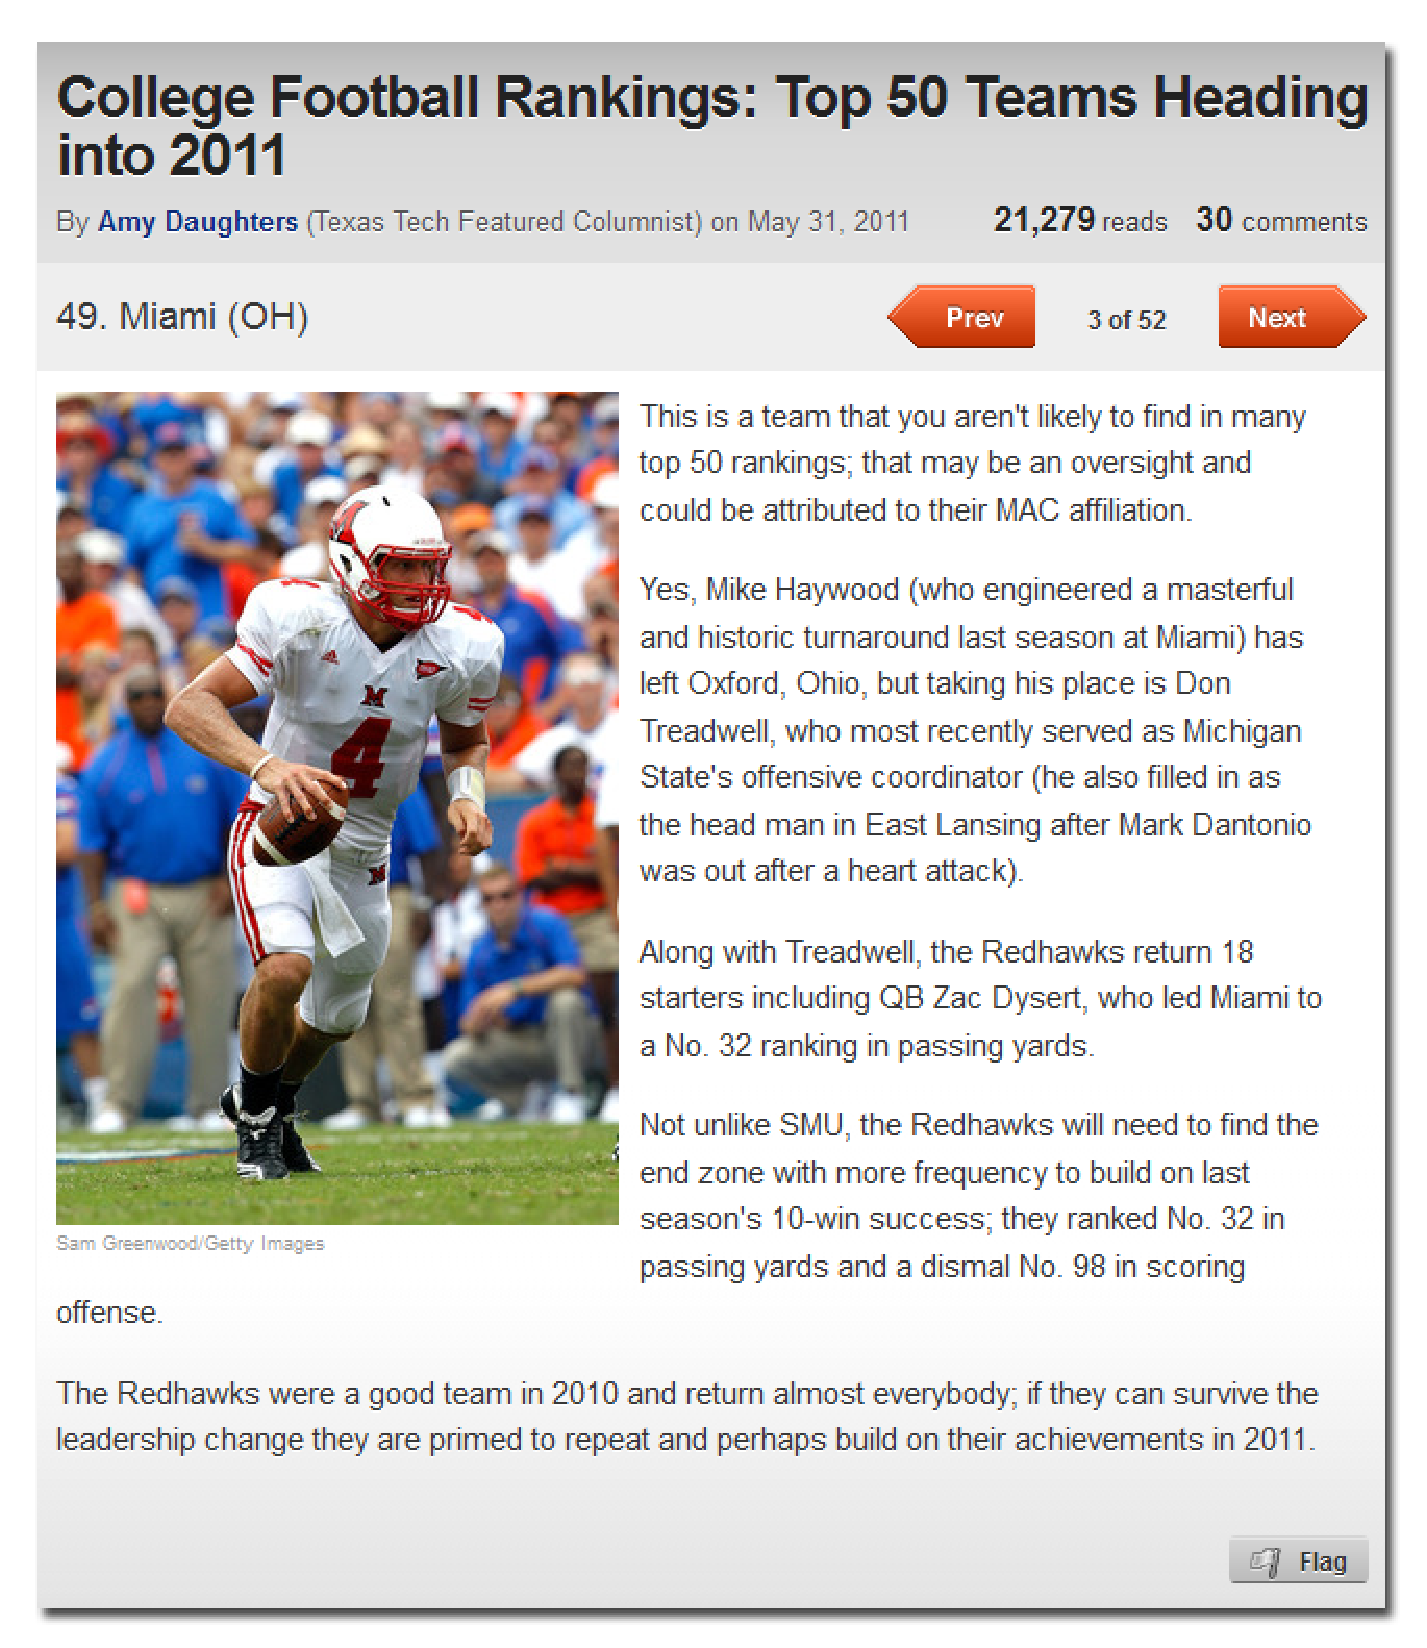
\epsfig{file=./pic/page4.eps, width=0.7\columnwidth}
%	\caption{Snapshot of a slide-show type top k page}
%	\label{fig:multipagelist}
%\end{figure}

The work described in this work is an important step in our bigger effort of
building an effective fact answer engine \cite{YinTL11:Facto}. 
With such an engine, we can answer queries such as
``Who are the 10 tallest persons in the world'', or ``What are 50 best-selling
books in 2010'' directly, instead of referring the users to a set of ranked
pages like all search engines do today. Because of the special relation
between the page title and the main list contained in the page, the semantics
of the list items are more specific and hence it's much easier for us to
integrate the extracted lists into a general knowledge base that empowers
the fact answer engine. 

%To that end, we have already built one of
%the largest open-domain taxonomy called Probase \cite{wentao} 
%which consists of 2.7 million concepts and many more instances. 
%However, that attempt primarily employs Hearst 
%patterns \cite{Hearst92} to extract concept-instance pairs from web text, and
%is unable to discover instances stored in structured web data such as
%lists. 

There were many previous attempts to extract lists or tables from the web.
None of them targets the top-k list extraction that is studied in
this work. In fact, most of the methods are based on either very specific
list-related tags \cite{googlesets,webtables08} 
such as {\tt <ul>}, {\tt <li>} and {\tt <table>} 
or the similarity between DOM trees 
\cite{LiuGZ03:MDR,MiaoTHSM09:TagPathClustering} and completely ignore
the visual aspect of HTML documents. These approaches are likely to be
brittle because of the dynamic and inconsistent nature of web
pages. More recently several groups
have attempted to leverage visual information in HTML in 
information extraction. Most notably, Ventex 
\cite{GatterbauerBHKP2007:Towards} and HyLiEn \cite{FumarolaWBMH11:List} 
are designed to correlate the rendered visual model or features
with the corresponding DOM structure and achieved remarkable improvements
in performance. However, these techniques indiscriminatingly extract {\em all}
elements of {\em all} lists or tables from a web page, therefore the objective
is different from that of this work which is to extract {\em one} specific
list from a page while purging all other lists (e.g. (d) and (e) in
Figure \ref{fig:topscientists}) as noise. The latter poses
different challenges such as distinguishing ambiguous list boundaries
and identifying noise and unwanted lists. 

 
%These techniques can hardly solve our problem for three reasons.
%First, these techniques focus on {\em deep web pages} 
%which are generated by backstage servers and data bases. 
%Thus, the list items in those pages are highly structured, 
%which makes list extraction relatively easy.
%When they turn to {\em top-k pages}, 
%it becomes more complicated as they are mostly edited manually.
%In fact, the effect of these methods reduce heavily when we use {\em top-k pages} as input.
%Second, these techniques merely retrieve all the lists in a page, 
%and fail to decide which one to be the top-k list.
%This is important for our problem 
%because it is common for a {\em top-k page} to contain other lists 
%like the lists showed in Figure \ref{fig:detailedWebPage} (d) and (e),
%which is irrelevant to the topic of page.
%Third, some of the techniques are not practicable for our problem,
%because the algorithms behind them are so complicated and time-consuming,
%that it may take too much time for analyzing a single page.

%The list extraction problem is challenging for the following reasons.
%First we should make sure our solution to have a satisfied outcome, 
%which is mainly indicated by the recall and precision value.
%This requires our approach to handle most cases, including some ``tricky'' ones.
%Second, we must offer a mechanism to value a few lists to pick up the right one
%(or to filter the noise lists).
%Third, it is not easy to get the exact name of the list items. For example, 
%the exact name of the list item shown in Figure \ref{fig:detailedWebPage} (b) should be ``Seychelles''.
%{\bf zzx's words here.}

The main approach of this work goes along the line of 
analyzing similar tag paths in the DOM tree with the help of
visual features to identify the main list in a page. 
The key contributions of this demo are:
\begin{itemize}
\item We defined a novel top-k list extract problem which is useful in
knowledge discovery and fact answering; 
\item We designed an unsupervised general-purpose algorithm along with
a number of key optimizations that is capable of extracting top-k 
lists from any web pages (in Section \ref{sec:algo});
\item Our evaluation shows that our algorithm scales with the data size
and achieves significantly better accuracy than competing methods
(in Section \ref{sec:eval}).
\end{itemize}
